\cotefile{123}
\scanpage{2}
Compléments sur transformation de Coxeter d'un système de racines\inserted{\handwritten{\unsure{irréductible|irreductible}}} (Kostant).
\margin{\handwritten{The principal 3-dimensional subgroup ....\quad th. 9.2.}}
% The insertion above the title is enclosed in an oval, with a leader to after ``racines''.
\margin{\handwritten{\figure{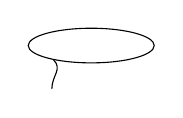
\begin{tikzpicture}[x=1cm,y=1cm]\draw (0,0) ellipse (0.8 and 0.22);\draw (-0.48,-0.18) .. controls (-0.36,-0.3) and (-0.5,-0.38) .. (-0.5,-0.55);\end{tikzpicture}}}}

a) Soit $w\handwritten{\in}W$. Alors toute valeur propre de $w$ \unsure{est} une racine de $1$ d'ordre divisant un des entiers $m_i+1$ (où les $m_i$ sont les exposants caractéristiques), donc d'ordre $\handwritten{\leq}h$. Pour qu'il y en ait une qui soit d'ordre $h$, il faut et il suffit que $w$ soit une transformation de Coxeter, et\inserted{alors} les éléments non nuls du sous-espace propre correspondant\inserted{\handwritten{(qui est de dim $1$)}} sont des éléments réguliers.
\margin{\handwritten{\figure{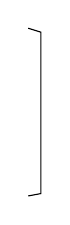
\begin{tikzpicture}[x=1cm,y=1cm]\draw (-0.16,0.05)--(0,0)--(0,-2.05)--(-0.16,-2.08);\end{tikzpicture}}}}

\uline{Corollaire}\handwritten{\unsure{1|!}}: Soit $\handwritten{\mu}$ le sous-groupe de $W$ engendré par un élément de Coxeter $c$, donc $\handwritten{\mu\simeq}\underline{Z}\handwritten{/}h\underline{Z}$. Alors $\handwritten{\mu}$ est égal au centralisateur de $c$, donc de $\handwritten{\mu}$, et si $\handwritten{\nu}$ est le normalisateur de $\handwritten{\mu}$, l'homomorphisme
\margin{\handwritten{\figure{\begin{tikzpicture}[x=1cm,y=1cm]\draw (0,0)--(0,-2.4);\end{tikzpicture}}}}
\[
\handwritten{\unsure{\nu|\psi}/\mu\longrightarrow}\operatorname{Aut}(\handwritten{\mu})\handwritten{\simeq}(\underline{Z}/h\underline{Z})^{\handwritten{*}}
\]
\margin{\handwritten{Quelle extension de $(\unsure{Z|\mathbb{Z}}/hZ)^*$ par $Z/hZ$ obtient-on ?}}
est \unsure{un} isomorphisme; en d'autres termes, pour tout entier $n$ premier à $h$, il existe un $w\handwritten{\in}W$ tel que $wcw^{-1}=c^h$, et $w$ est déterminé mod $\handwritten{\mu}$.
\margin{\handwritten{\unsure{échanger|échange} avec cor.\unsure{3|?}}}

Soit \unsure{en} ef\inserted{f}et $D$ \deleted{\unsure{une droite}}\inserted{le sous-espace} propre sous $c$ correspondant à une racine primitive $h$.ème de $1$. Alors $\dim D=1$ (prop.\handwritten{30}), et $\handwritten{z}=\operatorname{Centr}(\handwritten{\mu})$ normalise $D$, d'où un homomorphisme $\handwritten{z\to}\operatorname{Aut}(D)=\underline{C}^{\handwritten{*}}$, dont l'image est un sous-groupe fini de $\underline{C}^{\handwritten{*}}$, contenant l'image (isomorphe) de $\handwritten{\mu}$, donc cyclique d'ordre un multiple de $h$. Grâce à Kostant, son ordre est égal à $h$, et on a donc trouvé une rétraction $\handwritten{z\to\mu}$, il faut prouver que son noyau est réduit à $1$. Or si $w$ est dans ce noyau, il \deleted{induit} centralise $D$, et \unsure{qômme|comme} $D$ est régulière par Kostant,cela implique $w=1$. \unsure{On|Bn} a donc prouvé $\handwritten{z}=\handwritten{\mu}$. Reste à prouver que si $n$ est un entier premier à $h$, alors $c^n$ est conjugué de $c$, ce qui résulte également de Kostant.

\uline{Corollaire}. Soit $c$ un élément de Coxeter, et $\handwritten{\lambda}$ une valeur propre de $c$, correspondant à un vecteur propre $x$. Pour que $x$ soit régulier, il faut et il suffit que $\handwritten{\lambda}$ soit une racine primitive $h$.ème de $1$.
\margin{\handwritten{\figure{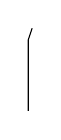
\begin{tikzpicture}[x=1cm,y=1cm]\draw (0.05,0)--(0,-0.15)--(0,-1.05);\end{tikzpicture}}}}

La suffisance a déjà été énoncée avec le th. de Kostant. Pour la nécessité, soit $h'\handwritten{\leq}h$ l'ordre de la valeur propre, alors $c^{h'}$ centralise $x$, donc, $x$ étant régulier, on a $c^{h'}=1$, donc $h'=h$, cqfd.

\uline{Corollaire}. \deleted{\unsure{Considérons}} \deleted{Soit $D$ une}\inserted{Soit $D$ une} droite régulières dans $V\unsure{\otimes|\mathbin{\text{\textcircled{x}}}}\underline{C}$ telle qu'il existe un élé%
% archive sheet number: 1
\scanpage{3}ment de Coxeter\inserted{$c$} de $W$ qui la normalise. Alors le normalisateur de $\unsure{\mathbb{D}|\deleted{W}D}$ dans $W$ est le groupe engendré par $c$, et il existe une unique élément de Coxeter de $W$ normalisant $D$ et y ayant pour valeur propre une racine \deleted{de}primitive donnée\inserted{$h$.ème} de $1$. Les droites régulières $D$ ayant la propriété précédente (appelées ``droites cycliques'' par Kostant) sont conjuguées sous $W$, leur nombre est égal à $\operatorname{card}(W)/h$.

NB Dans l'ensemble des droites cycliques, le groupe $(\underline{Z}/h\underline{Z})^{\handwritten{*}}$ opère\inserted{en commutant à l'action de $W$} librement; deux droites cycliques sont conjuguées sous l'action de ce groupe si et seulement si elles ont même stabilisateur dans $W$.
% archive sheet number: 2

\scanpage{16}
Résumé de quelques résultats de Kostant (sous groupes simples de rang $1$).

$G$ est un groupe semi-simple sur un corps $k$ de car. nulle, $\handwritten{\unsure{\mathfrak{g}|\mathscr{G}}}$ son algèbre de Lie.
\margin{\handwritten{(The principal 3-dimensional subgroup...., Am. Jour. Oct.1959, 3.4, 3.5, 3.6, \unsure{1.2|12}, 9.3)}}

\uline{Théorème} 1. \inserted{\handwritten{(i)}} Soient $x,e\handwritten{\in\mathfrak{g}}$,\inserted{(avec $e\handwritten{\ne}0$, $e$ nilpotent.\,)} Pour tout entier $k$, soit $\handwritten{\mathfrak{g}}(k)$ le sous-espace propre de\hspace{1.5em} correspondant à la valeur propre $k$. Donc si $x=\operatorname{Lie}(i)(1)$, où $i:\underline{G}_m\handwritten{\longrightarrow}G$, les $\handwritten{\mathfrak{g}}(k)$ sont les \deleted{décomposition} composants de $\handwritten{\mathfrak{g}}$ suivant les caractères de $\underline{G}_m$, opérant sur $\handwritten{\mathfrak{g}}$ via $i$ et la représentation adjointe. Les conditions suivantes sont \unsure{équivalentes}:

\[
\begin{aligned}
\text{a)}\quad &e\handwritten{\in\mathfrak{g}}(2)\quad\text{i.e.}\quad \handwritten{[}x,e\handwritten{]}=2e,\quad\text{et }\inserted{\text{pour tout entier }k\handwritten{\geq}1,}\\
&\operatorname{ad}(e)^k:\handwritten{\mathfrak{g}}(-k)\handwritten{\longrightarrow\mathfrak{g}}(k)\quad\text{est un isom}
\end{aligned}
\]

\[
\text{b)}\quad e\handwritten{\in\mathfrak{g}}(2),\quad\handwritten{\deleted{\unsure{et}}}\quad \operatorname{ad}(e):\handwritten{\mathfrak{g}}(0)\handwritten{\longrightarrow\mathfrak{g}}(-2)\quad\text{est surjectif},
\]
\inserted{\handwritten{et $x$ est de la forme $f(x_{\unsure{o|0}})$, par $f:\operatorname{Sl}(2,\unsure{k'|k})\to G$ (\uline{élément de Dynkin}).}}

\handwritten{\deleted{b') Comme b), avec $\operatorname{ad}(e):\mathfrak{g}(0)\to\mathfrak{g}(\unsure{2|-2})$ \uline{\unsure{bijectif}}}}

\[
\text{c)}\quad e\handwritten{\in\mathfrak{g}}(2),\quad\text{et }x\handwritten{\in}\operatorname{ad}(e)(\handwritten{\mathfrak{g}}).
\]

\[
\text{c')}\quad e\handwritten{\in\mathfrak{g}}(2),\quad\text{et }x\handwritten{\in}\operatorname{ad}(e)(\handwritten{\mathfrak{g}}(-2)).
\]

d) Il existe un homomorphisme $f:\operatorname{Sl}(2,k)\handwritten{\longrightarrow}G$ tel que $f^{\handwritten{'}}(e_o)=e,f^{\handwritten{\unsure{''|'}}}(x_o)=x\deleted{\unsure{y}}$ où $(x_o,e_o,f_o)$ est la base de $\operatorname{Lie}\operatorname{Sl}(2,k)$ correspondant à l'épinglage habituel de ce groupe.

C$\overset{\unsure{-}}{\underset{\text{\unsure{e}}}{\text{e}}}$s conditions impliquent \unsure{qu'il|qu'ib} existe un homomorphisme $i:\underline{G}_m\handwritten{\longrightarrow}G$, tel que $\operatorname{Lie}(i)(1)=x$, a fortiori que $x$ est semi-simple. De plus, le $f$ de d) est déterminé de façon unique.

(ii) Pour tout élément nilpotent $e$ de $\handwritten{\mathfrak{g}}$, il existe un \unsure{homomorphisme} $f:\operatorname{Sl}(2,k)\handwritten{\longrightarrow}G$ tel que $f(e_o)=e$, ou ce qui revient au même, tel que $f(u_o)=u$ (où $u=\exp(e)$, $u_o=\exp(e_o)$);\inserted{\handwritten{$f$ est uniquement déterminé \unsure{par} $x=f(x_o)$ i.e., par $i=f\circ i_o$.}} \unsure{En} vertu de (i), il revient au même,\deleted{\unsure{(}}lorsque $e=0$ i.e. $u\handwritten{\ne}1$, de dire qu'il existe un $x\handwritten{\in\mathfrak{g}}$ tel que $(x,e)$ satisfasse aux conditions équivalentes de (i), ou encore un homomorphisme $i:\underline{G}_m\handwritten{\longrightarrow}G$ tel que $(\operatorname{Lie}(i)(1),e)$ y satisfasse. Les homomorphismes $f$ en question sont conjugués \deleted{sous les éléments de}\inserted{par $\handwritten{Z=}$}$\operatorname{Cent}(e)=\operatorname{Cent}(u)$ (i.e. pour $e\handwritten{\ne}0$, les $x$ en question, ou encore les $i$ en question, sont conjugués \deleted{sous} par $\operatorname{Cent}(u)$), et lorsque $e\handwritten{\ne}0$, les \deleted{\unsure{morphismes}\quad $g$\quad $\operatorname{int}(g)$} $f$ en question (ou encore les
% archive sheet number: 15
\scanpage{17}
$x$ en question, ou les $i$ en question) forment un \uline{torseur} sous le groupe $\handwritten{Z^+}=$\deleted{$\handwritten{\unsure{U\cap}}\operatorname{Cent}(u)$}\inserted{$\handwritten{Z\cap U}$}, qui est un groupe unipotent\handwritten{.}
\margin{\handwritten{\deleted{(en fait, $\unsure{\subset|c}U$ introduit dans (iv))}}}
\margin{\handwritten{cf plus bas définition de $U$. On a $Z=Z_{\unsure{o|0}}.Z^+$ \deleted{\unsure{Commuté|Commutatif}} (produit semi-direct) avec $Z_o=Z\cap L=\operatorname{Cent}(f)$.}}
Enfin, supposant toujours $e\handwritten{\ne}0$, l'ensemble des $x$ en question est un torseur sous \deleted{$\handwritten{\unsure{\mathfrak{g}|\mathscr{G}}}^{e}=$ (centralisateur de $e$ \deleted{\unsure{dans}} dans $\handwritten{\mathfrak{g}}$)$=\operatorname{Ker}\operatorname{ad}(e)=\operatorname{Lie}\operatorname{Cent}(u)$}\inserted{$\handwritten{\operatorname{Lie}(Z^+)=\mathfrak{g}^{e}\cap\operatorname{Fil}^{1}(\mathfrak{g})}$} (\inserted{\handwritten{torseur}}pour l'addition, i.e. est de la forme $a+\handwritten{\mathfrak{g}}^e$, pour un $a\handwritten{\in\mathfrak{g}}$ convenable). \deleted{(et on a $\handwritten{\mathfrak{g}^{e}\subset\sum_{k\geq1}\mathfrak{g}}(k)=\operatorname{Fil}^{1}\handwritten{\mathfrak{g}}$)}

(iii) Soit $x\inserted{\handwritten{\ne0}}$ un élément de Dynkin de $\handwritten{\mathfrak{g}}$, donc associé à un homomorphisme de Dynkin $i:\underline{G}_m\handwritten{\longrightarrow}G$. Alors les éléments\inserted{\handwritten{$e$}} de $\handwritten{\mathfrak{g}}$ tels que $(x,e)$ satisfasse\deleted{nt} aux conditions de (i) forment un ouvert dense\inserted{\handwritten{\deleted{$\unsure{\mathfrak{g}(2)^*}$}}} de $\handwritten{\mathfrak{g}}(2)$ (savoir l'ouvert\inserted{\handwritten{$\mathfrak{g}(2)^*$}} des points $e$ tels que $\operatorname{ad}(e):\handwritten{\mathfrak{g}}(0)\handwritten{\to\mathfrak{g}}(2)$ soit surjectif), \deleted{qui}\inserted{\unsure{Celui+ci|Celui-ci}} est un \deleted{\uline{torseur}}\inserted{\handwritten{espace homogène}} sous\inserted{\handwritten{$L=$}}$\operatorname{Cent}(x)=\operatorname{Cent}(i)$, qui est un groupe réductif.

(iv) Bour tout \deleted{couple $(x,e)$ satisfaisant les conditions de (i),}\inserted{élément de Dynkin $x$ de $\handwritten{\mathfrak{g}}$, $x=\operatorname{Lie}(i)(1)$,} considérons les sous-groupes $P,U,\inserted{L}$ de $G$ définis par les conditions
\[
\operatorname{Lie}P=\handwritten{\sum_{k\geq0}\mathfrak{g}}(k)\quad,\quad
\operatorname{Lie}U=\handwritten{\sum}_{k\handwritten{\geq}\deleted{0}\handwritten{\unsure{1}}}\handwritten{\mathfrak{g}}(k),\quad
\operatorname{Lie}L=\handwritten{\mathfrak{g}}(0).
\]
Alors $P$ est un sous-groupe parabolique de $G$, $U$ est son radical unipotent, et $L=\operatorname{Cent}(x)=\operatorname{Cent}(i)$ \deleted{\unsure{en|un}} est un sous-groupe de Lévi de $G$. Si $\unsure{u|a}\inserted{=\exp(e)}$ est un élément unipotent de $G$ tel que $(i,u)$ soit un couple de Dynkin (i.e. induit par un $f:\unsure{\operatorname{SZ}|\operatorname{Sl}}(2,k)\handwritten{\to}G$), $P$ (donc \unsure{aassi|aussi} $U$) est défini en termes de $u$ (i.e; deux $x$ associés au même $u$ donnent le même $P$, cf. (ii)); il en est de même du sous-groupe $H=i(\underline{G}_m).U$ de $G$ (NB $i(\underline{G}_m)$ normalise $U$, et $H$ est un produit semi-direct), et de $i$ mod $U$ i.e. de $\underline{G}_m\handwritten{\longrightarrow}H/U$ induit par $i$. \unsure{De|Ae} plus, l'application
\[
g\handwritten{\longmapsto}\operatorname{ad}(g).x
\]
est un\deleted{e} isomorphisme de $U$ avec $x+\operatorname{Fil}^{1}\handwritten{\mathfrak{g}}\inserted{\handwritten{=x+\operatorname{Lie}U}}$ (où on pose $\operatorname{Fil}^{k}\handwritten{\mathfrak{g}}=\handwritten{\sum_{j\geq k}\mathfrak{g}}(j)$), et l'application
\[
g\handwritten{\longmapsto}\operatorname{ad}(g).\handwritten{e}
\]
est une application surjective de $U$ sur $e+\operatorname{Fil}^{\handwritten{3}}(\handwritten{\mathfrak{g}})$, ou de $P$ sur $\handwritten{\mathfrak{g}}(2)^{\handwritten{*}}+\operatorname{Fil}^{\handwritten{3}}(\handwritten{\mathfrak{g}})$, où $\handwritten{\mathfrak{g}}(2)^{\handwritten{*}}$ est l'ouvert de $\handwritten{\mathfrak{g}}(2)$ envisagé dans (iii).
% archive sheet number: 16

\scanpage{18}
\uline{Interprétations en termes de filtrations du foncteur oubli \deleted{sur la catégorie}} des représentations linéaires de dimension finie de $G$. (Il s'agit de filtrations compatibles au produit tensoriel\inserted{et ``exactes',cette \unsure{dernière} cond. aut. si $\operatorname{car}.k=0$}). Supposons fixé une classe\inserted{\handwritten{$c$}} de\inserted{conjugaison, rationelle sur $k$, de} telles filtrations (NB elle n'admet pas nécessairement un représentant rat/$k$); \unsure{il} revient au même de se donner,\deleted{un} pour le Chevalley $G_{\unsure{o|0}}$ associé à $G$, un \deleted{homomorphisme} élément de $\operatorname{Hom}(\underline{G}_m,T_o)/W=M/W$ ($T_o=M\unsure{\otimes|\mathbin{\text{\textcircled{x}}}}\underline{G}_m$ est le tore maximal type de $G_o$) invariant par le sous-groupe\inserted{\handwritten{$\Gamma$}} de $\operatorname{Auext}G_o=E_o$ image de $\operatorname{Gal}(\handwritten{\bar{k}}/k)$, ou encore un \deleted{homomorphisme $\underline{G}_m\unsure{\to}T$} élément de $M$ qui soit dans la chambre de Weyl de $M\otimes_{\underline{Z}}\underline{R}$ et qui soit stable par $\handwritten{\unsure{\Gamma'|\Gamma}}$. On a alors le \unsure{schéma} $\handwritten{\unsure{\underline{\phi}|\underline{\varnothing}}_c}$ des filtrations de classe $\handwritten{c}$, qui est un espace homogène sous $G$, de stabilisateur des points des paraboliques;\inserted{\handwritten{il} est\inserted{\handwritten{$\sim$}} un sous-schéma ouvert de $\uline{Par}(G)$, orbite rationelle sous $G$,\handwritten{soit $c'$,}} On peut regarder aussi le schéma $\operatorname{ST}_c$ des homomorphismes $i:\underline{G}_m\handwritten{\to}G$ de classe $c$, qui est donc une orbite rationelle de $G$ opérant sur $\uline{Homgr}(\underline{G}_m,G)$. Il est canoniquement isomorphe au schéma des couples de Lévi $(P,L)$ tels que $P$ soit de classe $c'$. (En d'autres termes, grâce au choix d'un $c$, pour $P$\inserted{ou encore $\handwritten{\underline{\phi}}$} de classe $c'$ donné, il revient au même de se donner un $i:\underline{G}_m\handwritten{\to}P$ de la classe définie par $c$, où un sous-groupe de Lévi de $P$, à $i$ étant associé $\operatorname{Cent}(i)$.\handwritten{)} On a \deleted{\unsure{un homo}}\inserted{deux}morphismesde schémas canoniquement isomorphes
\[
\operatorname{ST}_c\handwritten{\longrightarrow\underline{\phi}}_c\quad,\quad
(\operatorname{CL})_{c'}\handwritten{\longrightarrow}\operatorname{Par}_{c'}\quad,
\]
le premier en termes de théorie des filtrations \unsure{da|du} foncteurs fibres, le deuxième \deleted{\unsure{d}}en termes de groupes paraboliques.

Supposons maintenant que $k$ soit de car. nulle (j'ignore dans quelle mesure c'est vraiment nécessaire). On peut alors considérer le Schéma $\operatorname{Dyn}_c$ des homomorphismes $f:\operatorname{Sl}(2,k)\handwritten{\longrightarrow}G$ tels que $fi_o$ soit de classe $c$. Supposons-le non vide\inserted{\handwritten{et non réduit à un point,}} i.e. $c$ une classe de Dynkin\inserted{\handwritten{$\ne1$}}. Alors $\operatorname{Dyn}_c$ est un \deleted{\uline{torseur}}\inserted{\handwritten{espace homogène}} sous $G$\inserted{\handwritten{de stabilisateur $Z_o$ (il faudrait regarder la structure de ces $Z_o$; dimension, semi-simplicité).}}\deleted{(en fait, il est can. is. au torseur $\uline{Isom}(G_1,G)$, où $G_1$ est le groupe quasi-déployé correspondant à $G$).} Soit $\operatorname{Un}_c$ le schéma des éléments unipotents\inserted{\handwritten{de $G$}} dont la classe corresponde à \deleted{celle de} $c$ par la correspondance
% archive sheet number: 17
\scanpage{19}
de Kostant. On a donc des morphismes $f\handwritten{\unsure{\mathrel{\mapstochar\relbar}|\mapsto}}f\handwritten{\circ}i_{\unsure{o|0}}$ et $f\handwritten{\mathrel{\mapstochar\relbar}}f(u_o)$ de $\operatorname{Dyn}_c$ dans $\operatorname{ST}_c$ resp. $\operatorname{Un}_c$. D'autre part, Deligne nous fournit $\operatorname{Un}_c\handwritten{\to\unsure{\underline{\phi}|\underline{\varnothing}}}_c$, et celui-ci peut aussi être défini par la commutativité du diagramme \handwritten{d'esp. homogènes}
\diagram{\begin{tikzcd}[ampersand replacement=\&]
\operatorname{ST}_c\handwritten{\simeq}(\operatorname{CL})_{c'} \handwritten{\arrow[d]} \& \operatorname{Dyn}_c \handwritten{\arrow[l]} \handwritten{\arrow[d]} \\
\handwritten{\underline{\phi}}_c\handwritten{\simeq}\operatorname{Par}_{c'} \& \operatorname{Un}_c \handwritten{\arrow[l]}
\end{tikzcd}}
\margin{\handwritten{\diagram{\begin{tikzcd}[ampersand replacement=\&,column sep=small,row sep=small]
L \arrow[d] \& Z_o \arrow[l] \arrow[d] \\
P \& \unsure{z(e)|Z(e)|\mathfrak{z}(e)} \arrow[l]
\end{tikzcd}}}}
.

Pour qu'il existe un point rationnel de \deleted{$\operatorname{Dyn}_c$, ou ce qui revient au même} $\handwritten{\underline{\phi}}_c\handwritten{\simeq}\operatorname{Par}_{c'}$, il faut (et suffit) qu'il en existe un de $\operatorname{Dyn}_c$ \deleted{i.e. que $G$ soit quasi-déployé}\inserted{\handwritten{(i.e., si $Z_o=e$, que $G$ est quasi-déployé)}}: en effet, $P$ étant choisi, \deleted{\unsure{ceci}} on peut en choisir un \deleted{point rationnel} sous-groupe de Lévi $L$,\deleted{i.e.}\inserted{\handwritten{ou ce qui revient au même}} un $i:\underline{G}_m\handwritten{\to}G$ dans la classe $c$,définissant $P$, et alors les $u=\exp(e)$ qui \deleted{aux} s'adaptent à $i$ forment un ouvert dense de $\handwritten{\unsure{\mathfrak{g}|\mathscr{G}}(2)}$, qui \deleted{est donc non vide} a donc un point rationnel. On voit donc que pour certaines classes de paraboliques (qu'on pourrait appeler les paraboliques de \inserted{Dynkin-}Kostant\unsure{)} l'existence d'un parabolique de cette classe rationnel sur $k$ implique déjà que $G$ est quasi-déployé. (NB Quand $G$ n'est pas une forme intérieure, il faut faire attention cependant de vérifier d'abord que la classe $c'$ de $P$ provient bien d'un $c$ de Dynkin \uline{invariant par} $\handwritten{\Gamma}$, et il n'est pas clair que cette propriété\inserted{de $c$} résulte du fait que $c'$ est \unsure{invariantè|invariante} par $\handwritten{\Gamma}$, faute de savoir si $c\handwritten{\mapsto}c'$ est injectif sur les classes de Dynkin). \handwritten{(}On notera aussi que l'argument donné \deleted{\unsure{p}}marche également sur un anneau semi-local (de car. nulle jusqu'à nouvel ordre).\handwritten{)}
\margin{\handwritten{\unsure{Il|Ce} n'est en effet pas le cas, p.ex. pour $A_2,A_4$ (cela l'est pour $A_3$)}}
Ceci montre l'intérêt, pour des questions arithmétiques, de déterminer exactement les\inserted{classes \handwritten{de}} sous-groupes parab\handwritten{\unsure{-}}oliques de Dynkin-Kostant des divers groupes simples, et de voir si: leur stabilisateur dans $\operatorname{Autext}(G_o)$ est le même que celui des $c$ de Dynkin correspondants, et pas str. plus grand.

On notera cependant que si une filtration du foncteur \deleted{fib} oubli peut être définie par un élément unipotent, la classe de conjugaison de ce der%
% archive sheet number: 18
\scanpage{20}nier (ou, ce qui revient au même, $c$) est bien déterminée. Les unipotents qui définissent ladite filtration, en termes d'un $i$ qui la définit, sont\inserted{ceux} de la forme $\exp(e)$, où $e$ parcourt $\handwritten{\unsure{\mathfrak{g}|\mathscr{G}}}(2)^{\handwritten{*}}+\operatorname{Fil}^{\handwritten{3}}(\handwritten{\mathfrak{g}})$. Ils forment une classe de conjugaison d'éléments de $U$ \uline{par} $P$ (NB mais pas par $U$), les classes de conjugaison \uline{par} $U$ s'identifiant aux ensembles de la forme $(\exp(e)\handwritten{\mid}e\handwritten{\in}a+\operatorname{Fil}^{\handwritten{3}}(\handwritten{\mathfrak{g}},))$, où $a\handwritten{\in\mathfrak{g}}(2)^{\handwritten{*}}$ est un élément quelconque.\deleted{de}

\uline{Cas principal}. Pour qu'on ait\hspace{1.5em}$(1)=0$, il faut et suffit que \deleted{l'homomor} la classe d'homomorphismes $f:\operatorname{Sl}(2,k)\hspace{1.5em}G$ envisagée soit ``\unsure{principale}'' au sens de Dynkin-Kostant. Alors le parabolique associé $P$ est un Borel (la réciproque n'étant pas vraie \deleted{sans doute}, cf table de Dynkin), et le groupe $Z_{\unsure{o|0}}$ est le groupe unité (i.e. $\operatorname{Dyn}_c$ est un torseur sous $G$), \unsure{la} réciproque n'étant pas vraie sans doute.
\margin{\handwritten{\uline{ex}\quad Cas $A_2,A_4$ les paraboliques associés aux unipotents ``sous-réguliers'' sont des \unsure{Borels|borels} !}}
% archive sheet number: 19
